\documentclass[10pt, compress]{beamer}

\usetheme{glasgow}

\usepackage{booktabs}
\usepackage[scale=2]{ccicons}
\usepackage{minted}

\usepgfplotslibrary{dateplot}

\usemintedstyle{trac}

% Specifiy the location of images to be used
\graphicspath{{src/}}

%% Customisation
% \newcommand{\V}[1]{\v} % vectors \v{c}
% \renewcommand{\v}[1]{\mathbf{#1}} % vectors
\newcommand{\ti}[1]{\tilde{#1}} % spectral representation
\newcommand{\tnsr}[1]{\underline{\underline{#1}}}

% Symbols
\renewcommand{\O}{\omega}  % omega
\newcommand{\E}{\varepsilon}  % epsilon
\renewcommand{\u}{\mu}  % mu
\newcommand{\p}{\rho}  % rho
\newcommand{\x}{\times}  % times
\renewcommand{\inf}{\infty}  % infinity
\newcommand{\infint}{\int\limits_{-\inf}^\inf} % integral by R
\newcommand{\e}{\mathrm{e}} % Straight-up exponential
\renewcommand{\j}{{j}\mkern1mu} % Straight-up exponential
\newcommand{\iu}{\mathrm{i}\mkern1mu}

\newcommand\ddfrac[2]{\frac{\displaystyle #1}{\displaystyle #2}}





\title{High Frequency Communication Systems}
\subtitle{Lecture 2}
\date{Spring 2021}
\author{Hasan Abbas \& Qammer Abbasi}
% \institute{}

\begin{document}

\maketitle

%%%%%%%%%%%%%%%%%%%%%%%%%%%%%%%%%%%%%%%%%%
%%%%%%%%%%%%%%%%%%%%%%%%%%%%%%%%%%%%%%%%%%
%%%%%%%%%%%%%%%%%%%%%%%%%%%%%%%%%%%%%%%%%%
\begin{frame}[fragile]
  \frametitle{Lecture Outline}
\begin{outline}[itemize]
  \1 Plane waves and the wave equation
  \1 Dielectric Properties and Materials
  \1 \color{red}{Nanoscale Electromagnetics}
\end{outline}
\end{frame}
%%%%%%%%%%%%%%%%%%%%%%%%%%%%%%%%%%%%%%%%%%
%%%%%%%%%%%%%%%%%%%%%%%%%%%%%%%%%%%%%%%%%%
%%%%%%%%%%%%%%%%%%%%%%%%%%%%%%%%%%%%%%%%%%
\begin{frame}[fragile]
\frametitle{The Wave Equation}
\begin{outline}
  \1 Maxwell's Equations are first-order partial differential equations
    \2 They are coupled equations (i.e. the unknown $\va{E}$ and $\va{H}$) appear in each equation
  \1 To find the solution of the equations we treat it as a boundary value problem
  \1 We also uncouple the equations by raising the order (\textit{here two}).
  \1 The result is the \textit{wave equation}.
\end{outline}
\end{frame}



\begin{frame}[fragile]
  \frametitle{The Vector Wave Equation}
Recall,
\begin{align*}
  \curl \va{E} &= -\u \pdv{\va{H}}{t} - \va{M} \tag{Faraday's Law}\\
\curl \va{H} &= \pdv{\va{D}}{t} + \va{J} \tag{Ampere's Law} \\
\end{align*}
where,
\begin{align*}
  \va{J} &= \va{J}_i + \sigma \va{E}
\end{align*}
We take the curl of the above two equations and use the vector identity, $\curl \curl \va{A} \equiv \grad{(\div \va{A})} - \laplacian{\va{A}}$,
\begin{align*}
  \grad{(\textcolor{red}{\div \va{E}})}   - \laplacian{\va{E}} &= - \curl{\va{M}} - \u \pdv{t}
  \left( \textcolor{red}{\curl{\va{H}}}  \right)  \\
  \grad{(\p_s /\E)} - \laplacian{\va{E}} &= -\curl{\va{M}} - \u \pdv{\va{J}_i}{t} - \u \sigma \pdv{\va{E}}{t} - \u \E \pdv[2]{\va{E}}{t}
\end{align*}
\end{frame}



\begin{frame}
  \frametitle{The Wave Equation - contd.}
  After rearranging we get the \textit{uncoupled} second-order differential equation for $\va{E}$,
  \begin{align*}
  \laplacian {\va{E}} &= \curl {\va{M}_i} + \u  \pdv{\va{J}_i}{t} + \u \sigma \pdv{\va{E}}{t} + \u \E \pdv[2]{\va{E}}{t} + \frac{1}{\E} \grad{\p_s}
  \end{align*}
  \begin{tcolorbox}[colback=blue!5,colframe=university-blue,title=Homework]
  \begin{outline}
    \1 Derive the vector wave equation for the magnetic field $\va{H}$
    \1 \textcolor{red}{Due on MS Teams on March 23.}

    \1 You can either scan your work or better typeset in \LaTeX.
  \end{outline}
\end{tcolorbox}
\end{frame}



\begin{frame}[fragile]
  \frametitle{Uniform Plane Wave}
      \begin{outline}
        \1 Simplest electromagnetic wave
        \1 Generally propagate in a fixed direction (e.g. $z$)
        \1 The EM fields are only functions of time and space coordinate $z$.
        \1 No variation in transverse coordinates ($\pdv{x}, \pdv{y} = 0$)
        \2 $E_z = H_z = 0$
        \end{outline}
        \begin{align*}
          \va{E}(x,y,z,t) = \va{E}(z,t)
        \end{align*}
\end{frame}
%%%%%%%%%%%%%%%%%%%%%%%%%%%%%%%%%%%%%%%%%%
%%%%%%%%%%%%%%%%%%%%%%%%%%%%%%%%%%%%%%%%%%
%%%%%%%%%%%%%%%%%%%%%%%%%%%%%%%%%%%%%%%%%%
\begin{frame}[fragile]
  \frametitle{Revisiting Maxwell's Equations}
  For a uniform plane wave, the source-free Maxwell's equations are:
  \begin{align*}
\curl \va{E} &= - \pdv{\va{B}}{t} \implies \vu{z} \cross \pdv{\va{E}}{z} = - \pdv{\va{B}}{t} \\
\curl \va{H} &= \pdv{\va{D}}{t}  \implies \vu{z} \cross \pdv{\va{H}}{z} =  \pdv{\va{D}}{t} \\
\div \va{E} &= 0  \implies \pdv{{E_z}}{z} = 0\\
\div \va{H} &= 0 \implies \pdv{{H_z}}{z} = 0
\end{align*}
  \end{frame}
%%%%%%%%%%%%%%%%%%%%%%%%%%%%%%%%%%%%%%%%%%
%%%%%%%%%%%%%%%%%%%%%%%%%%%%%%%%%%%%%%%%%%
%%%%%%%%%%%%%%%%%%%%%%%%%%%%%%%%%%%%%%%%%%

%%%%%%%%%%%%%%%%%%%%%%%%%%%%%%%%%%%%%%%%%%
%%%%%%%%%%%%%%%%%%%%%%%%%%%%%%%%%%%%%%%%%%
%%%%%%%%%%%%%%%%%%%%%%%%%%%%%%%%%%%%%%%%%%
\begin{frame}
  \frametitle{The Wave Equation - Plane Waves}
  \begin{outline}
    \1 Starting with a uniform plane wave in a source-free region.
    \1 Considering one-dimensional case
    \1 Since $E_z, H_z = 0$, we start with and use the identity ($\vu{z} \cdot (\vu{z} \cross \va{A}) \equiv 0$):
  \end{outline}
      \begin{align*}
        \vu{z} \cdot \qty( \vu{z} \cross \pdv{\va{H}}{z}) &= \E \pdv{\va{E}}{t} = 0 \implies \pdv{E_z}{t} = 0
      \end{align*}
      The solutions (transverse fields) must be of the form:
      \begin{align*}
        \va{E} \qty(z, t) = \vu{x} E_x \qty(z,t) + \vu{y} E_y\qty(z,t) \\
        \va{H} \qty(z, t) = \vu{x} H_x \qty(z,t) + \vu{y} H_y \qty(z,t)
      \end{align*}
      The electric and magnetic fields only exist in the $x-y$ plane which is \color{red}{perpendicular} to the direction of propagation.
 \end{frame}
%%%%%%%%%%%%%%%%%%%%%%%%%%%%%%%%%%%%%%%%%%
%%%%%%%%%%%%%%%%%%%%%%%%%%%%%%%%%%%%%%%%%%
%%%%%%%%%%%%%%%%%%%%%%%%%%%%%%%%%%%%%%%%%%
\begin{frame}
  \frametitle{The Wave Equation for Plane Waves}
  \begin{outline}
    \1 We can also simplify 1D Maxwell's equations
  \end{outline}
  \begin{align*}
    \vu{z} \cross \pdv{\va{E}}{z} &= -\frac{1}{c} \eta \pdv{\va{H}}{t} \\
        \eta \vu{z} \cross \pdv{\va{H}}{z} &= -\frac{1}{c} \pdv{\va{E}}{t}
  \end{align*}
  where,
  \begin{align*}
    c = \frac{1}{\sqrt{\u \E}}, and \eta = \sqrt{\frac{\u}{\E}}
  \end{align*}
  Using the BAC-CAB ($\va{A} \cross(\va{B} \cross \va{C})=\va{B}(\va{A} \cdot \va{C})-(\va{B} \cdot \va{A}) \va{C}$) rule of vector algebra:
  \begin{align*}
    \left( \vu{z} \cross \pdv{\va{E}}{z} \right) \cross \vu{z} &= \pdv{\va{E}}{z} (\vu{z} \cdot \vu{z}) - \vu{z} \left (\vu{z} \cdot \pdv{\va{E}}{z} \right) = \pdv{\va{E}}{z}
  \end{align*}
\end{frame}


\begin{frame}
  \frametitle{1D Wave Equation}
  We can now write the Maxwell's equations as:
  \begin{align*}
     \pdv{\va{E}}{z} &= - \frac{1}{c} \pdv{t} \left( \eta \va{H} \cross \vu{z} \right) \\
     \pdv{z} \left( \eta \va{H} \cross \vu{z} \right) &= -\frac{1}{c} \pdv{\va{E}}{t}
      \end{align*}

    We differentiate the first equation w.r.t $z$ and use the second:
    \begin{align*}
      \pdv[2]{\va{E}}{z} &= - \frac{1}{c} \pdv{}{t}{z} \left( \eta \va{H} \cross \vu{z} \right) = \frac{1}{c^2} \pdv[2]{\va{E}}{t}
    \end{align*}
    which is the 1D wave equation. We can also write in a convenient form as:
    \begin{tcolorbox}
      \begin{align*}
      \left( \pdv[2]{z} - \frac{1}{c^2} \pdv[2]{t}\right) \va{E} (z,t) = 0
    \end{align*}
    \end{tcolorbox}
\end{frame}

\begin{frame}
  \frametitle{Time-harmonic Wave Equation}
  \begin{outline}
    \1 Time-harmonic representation $\exp (\j \O t)$ is convenient in finding the solutions
    \1 We replace the derivatives $\pdv{t}$ and $\pdv[2]{t}$ by $\j \O$ and $-\O^2$ respectively
    \1 We also call the result as the \textcolor{red}{Helmholtz equation}.
    \1 For source-free ($\va{J} = \va{M} = 0$) case, we get
  \end{outline}
  \begin{align*}
    \laplacian{\va{E}} + \O^2 \u \E \va{E} &= 0 \\
    \laplacian{\va{E}} + \beta^2 \va{E} &= 0
  \end{align*}
  \end{frame}

  \begin{frame}
  \frametitle{Solutions to Wave Equations}
  \begin{outline}
    \1 A second order differential equation leads to 2 solutions
    \2 We can split the fields into \textit{forward} and \textit{backward} components.
    \1 We use the \textit{Separation of variables} method to obtain the solutions of vector wave equation
    \2 By solving the scalar equations for each components
  \end{outline}
  \begin{align*}
    \va{E} = \vu{x} E_x + \vu{y} E_y + \vu{z} E_z
  \end{align*}
  As an example, for the x-component, we get:
  \begin{align*}
    \laplacian{E_x}\left(x,y,z \right) + \beta^2 {E_x}\left(x,y,z \right) &= 0
  \end{align*}
  The solution is of the form:
  \begin{align*}
    E_x \left(x,y,z \right) &= f(x)g(y)h(z)
  \end{align*}
  \end{frame}


  \begin{frame}
  \frametitle{Solutions to Wave Equations}
  \begin{outline}
    \1 There are different forms of solutions we can use
    \2 Depends on the nature of the problem
    \1 For free-space problems, we use the travelling wave form
  \end{outline}
  \begin{align*}
    h(z) &= A_1 \exp \left(-\j \beta_z z \right) + B_1 \exp \left(+\j \beta_z z \right)
  \end{align*}
  For confined problems (such as a waveguide), we use the standing wave form:
  \begin{align*}
    g(x) &= A_2 \sin(\beta_y y) + B_2 \cos(\beta_y y)
  \end{align*}
  \end{frame}


\begin{frame}
  \frametitle{Plane Wave}
        \begin{outline}
        \1 Uniform travelling wave in the $+z$ direction
        \1 Equiphase plane (increase in $t$ also increase $z$)
      \end{outline}
    \begin{figure}[t!]
  \centering
        {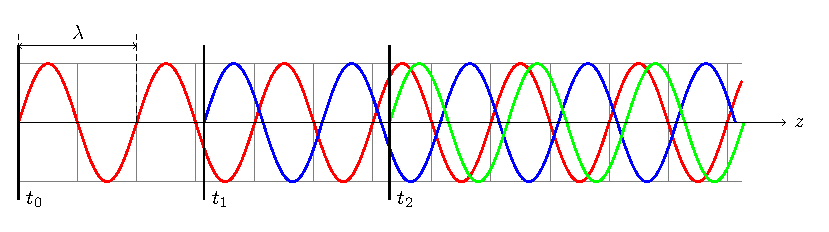
\includegraphics[scale=.8]{wave_eq.tex}
        \label{fig:EM}}
        \caption{X-polarized Plane Wave propagation along $z$ direction}
      \end{figure}
      For the above, the plane wave can be described as:
      \begin{align*}
        E_x (z,t) &= \cos(\O t - \beta z)
      \end{align*}
\end{frame}
\section{Material Properties}
\begin{frame}
      \frametitle{Modelling Material Properties}
      \begin{outline}
        \1 Materials play a huge role in electromagnetic radiation and guiding
        \1 The electrons inside the atom of a material behave differently when an external electric field is applied
        \2 The electric field distorts the electron distribution
        \2 An electric dipole moment is created
        \1 We tend to observe it macroscopically (not at the atom level but over the volume of the material)
        \1 We need to describe the behaviour of $\E$ with frequency (using Classical Harmonic model)
      \end{outline}
      \begin{align*}
        \dv[2]{x}{t} + \gamma \dv{x}{t} + \O_0^2 x &= \frac{e}{m} E
      \end{align*}
      where $\gamma$ is a measure of rate of collisions per unit time, $\O_0$ refers to the resonant frequency, $e$ and $m$ are the electron charge and mass respectively.
    \end{frame}


\begin{frame}
  \frametitle{Dielectric Models}
  \begin{outline}
    \1 Using the phaser form of the Harmonic model for a plane wave, $E(t) = E_0 \exp(\j \O t)$
  \end{outline}
  \begin{align*}
    \E(\O) &= \E_0 + \frac{\E_0 + \O_p^2}{\O_0^2 - \O^2 + \j \O \gamma} \tag{Lorentz Model}
  \end{align*}
  where $\E_0$ is the free-space permittivity, $\O_p$ is the plasma frequency given by:
  \begin{align*}
      \O_p &= \sqrt{\frac{Ne^2}{\E_0 m}}
  \end{align*}
  $N$ being the charge density. 
  \begin{outline}
    \1 The real part of $\E$ refers to the refractive properties
    \1 The imaginary part determines the absorption or loss.
  \end{outline}
\end{frame}

\begin{frame}
  \frametitle{Polarisation of Dielectrics}
  \begin{outline}
    \1 Formation of electric dipoles in the presence of external electric fields.
    \1 There are magnetic materials as well but we are not interested in them in this course.
    \2 We assume $\u_r = 1$ for all materials.
  \end{outline}
\begin{figure}
  \centering
  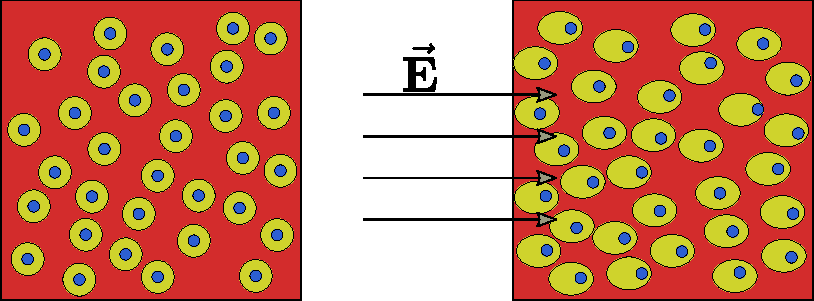
\includegraphics[scale=.6]{model.pdf}
  \caption{Effect of electric field on dipole formation.}
\end{figure}  
\end{frame}

\begin{frame}
  \frametitle{The Lorentz Function}
\begin{figure}[t!]
  \centering
        {\includegraphics[scale=.8]{lorentz.tex}
        \label{fig:lorentz}}
        \caption{The dielectric function using the Lorentz Model}
      \end{figure}
\end{frame}


\begin{frame}
  \frametitle{Conductors} 
  \begin{outline}
    \1 Main difference from dielectrics is that the motion of electric charges and the  generation of current flow.
    \1 Conductors have \textit{loosely held} electrons in the valence band of atoms \textcolor{red}{[free electrons]}
    \1 Conductors have very high values of electric conductivity ($\sigma \to \inf$).
    \1 For perfect electric conductors, we use $\sigma = \inf$.
  \end{outline} 
    \begin{align*}
    \E (\O) &= \E_0 + \frac{\sigma (\O)}{\j \O} \tag{Drude Model}
  \end{align*}
  % \begin{align*}
  %   t_r &= \frac{\E}{\sigma} = \frac{\SI{8.845e-12}{\F \per \m}}{\SI{5.76e7}{\siemens \per \m}} = \SI{1.54e-19}{\s}
  % \end{align*}
\end{frame}

\begin{frame}
  \frametitle{Plasmas}
  \begin{outline}
    \1 Plasma like solid, liquid and gas is the fourth form of matter
    \1 We consider the resonant frequency $\O_0 = 0$.
    \1 Plasma effectively acts as a switch
      \2 Before plasma frequency, wave is completely attenuated.
      \2 After $\O_p$, there is zero attenuation
  \end{outline}
  \begin{align*}
    \E (\O) &= \E_0 + \left( 1 - \frac{\O_p^2}{\O^2} \right)
  \end{align*}
\end{frame}


\section{Nanoscale Electromagnetics}
\begin{frame}
  \frametitle{Nanoscale Electromagnetics}
  \begin{outline}
    \1 Electronic device sizes are fast approaching the nanoscale
    \2 Modern transistors are typically \SI{5}{\nm} in size
    \1 Maxwell's equations have remained valid at macro scale
    \2 However, discrepancies have lately surfaced at the nanoscale level between the theory and experiment
    \1 Highlight of nanoscale electromagnetics is the \textit{complex-valued} nature of the relative permittivity
    \1 Interestingly, EM surface waves exist at metal/dielectric interfaces
  \end{outline}
  \begin{figure}
    \centering  
    {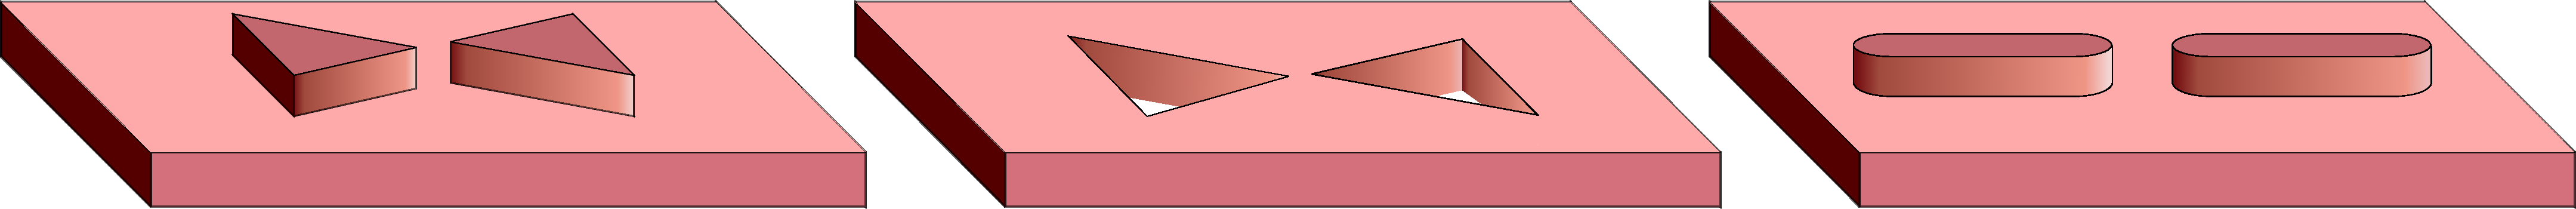
\includegraphics[width=.9\textwidth]{nanoantennas.pdf}}
  \end{figure}
\end{frame}


\begin{frame}
  \frametitle{Surface Plasmon Polaritons}
  \begin{outline}
    \1 EM fields can be split into \textit{transverse-magnetic} (TM) and \textit{transverse-electric} (TE) components
    \1 Observing a planar dielectric-metal interface, TM-mode means H-field only has a transverse ($H_y$) component
    \2 The E-field has $E_x$ and $E_z$ components
  \end{outline}
\end{frame}

\begin{frame}
  \frametitle{Surface Plasmons}
  \begin{outline}
    \1 At optical and mid infrared frequencies ( $>$ \SI{10}{\tera \hertz}), some materials such as gold exhibit negative dielectric constant $(\Re(\E_r) < 0)$ 
    \1 At a metal-dielectric interface such as the one below:
  \end{outline}
  \begin{figure}
    \centering 
  \def\svgwidth{.75\linewidth}
    \input{src/interface.pdf_tex}
  \end{figure}
\end{frame}


\begin{frame}
  \frametitle{Existence of Surface Plasmons}
  \begin{outline}
    \1 The TM mode fields in region 1 are expressed as:
  \end{outline}
      \begin{align*}
    \va{E}_1 ={}& \left(\vu{x} E_{x1}  + \vu{z} E_{z1}  \right) \, \exp \left( - \j (k_x x \,+\, k_{z1} z) \right), \\
    \va{H}_1 ={}& \vu{y} H_{y1}  \, \exp \left( - \j (k_x x \,+\, k_{z1} z) \right)
  \end{align*}
  and likewise for region 2. Using the Ampere's Law ($\curl \va{H} = -\j \O \va{E}$), we get the boundary conditions:
    \begin{align*}
    k_{z1} H_{y1} ={}& \O \E_1 E_{x1}\\
    k_{z2} H_{y2} ={}& -\O \E_2 E_{x2}
  \end{align*}
\end{frame}

\begin{frame}
  \frametitle{The Dispersion Relation}
  \begin{outline}
    \1 Ensuring the continuity of tangential fields, $E_{x1} = E_{x2}$ and $H_{y1} = H_{y2}$, we get:
    \end{outline}
    \begin{align*}
  \frac{k_{z1}}{\E_1} + \frac{k_{z2}}{\E_2} &= 0.
\end{align*}
\begin{outline}
  \1 Using the Helmholtz equation, ($\laplacian \va{E} + k_i^2 \va{E} = 0$) , where $i = 1,2$, and assuming the permeabilities of all regions are that of air, we obtain,
\end{outline}
\begin{align*}
  k_x &= k_0 \sqrt{\frac{\E_{r1} \E_{r2}}{\E_{r1} + \E_{r2}}}
\end{align*}
\end{frame}

\begin{frame}
  \frametitle{Visualising the Surface Plasmons}
  \begin{outline}
    \1 The dispersion relation has a solution when 
  \end{outline}
    \begin{equation*}
    \E_1 > 0, \quad    \E_2' < 0, \quad   \text{and}  \quad \left| \E_2' \right| > \E_1,
  \end{equation*}
  \begin{figure}[b!]
  \centering
  \def\svgwidth{.75\linewidth}
  \input{src/spp.pdf_tex}
  \caption*{Surface plasmon propagation along a dielectric-metal boundary and exponential decay perpendicular to the boundary.}
\end{figure}
\end{frame}
% \begin{frame}
%   \frametitle{Conductor Models}
%   \begin{figure}
%   \centering
%   \subfloat[Normal]{\animategraphics[loop,controls,width=.3\linewidth]{30}{Normal-}{0}{71}}
%   \subfloat[Resonance]{\animategraphics[loop,controls,width=.3\linewidth]{30}{Resonance-}{8}{49}}
%   \subfloat[High]{\animategraphics[loop,controls,width=.3\linewidth]{30}{High-}{0}{14}}     
% \end{figure}
% \end{frame}
\end{document}
